\section{Network Robustness}
\label{evaluation-sec-robustness}

The first evaluation metric that we consider is the {\em robustness} of the
sensor network.  Sensor network deployments have typically been plagued by
failures of individual nodes and the support infrastructure. Clearly,
robustness has a direct effect on the resulting data yield.  Our evaluation
shows that while nodes exhibited very high uptimes, the base station
infrastructure was very unreliable, and a single bug affecting the Deluge
protocol caused a three-day outage of the entire network.

%For example, in the 2003~Great Duck Island
%deployment~\cite{gdi-sensys04}, burrow nodes in the multihop network 
%failed after an average of 29~days, primarily due to battery
%exhaustion.

\subsection{Overall network uptime}

\begin{figure}[t]
\label{evaluation-fig-nodesalive}
\begin{center}
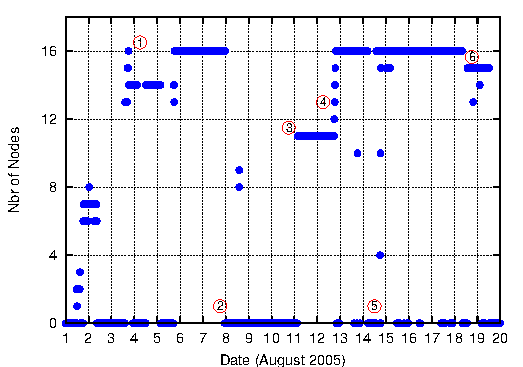
\includegraphics[width=\hsize]{./5-evaluation/figs/robustness/nodesalive/nodesalive.pdf}
\end{center}
\caption{\textbf{Nodes reporting over time.}
This figure shows the number of nodes reporting over each 10~min window
during the 19-day deployment period.  The annotations (1) through (6) are
described in the text.}
\end{figure}

Figure~\ref{evaluation-fig-nodesalive} shows the number of nodes reporting
over each 10-minute interval during the entire 19-day deployment. A node is
included in the count if any of its status messages were received at the base
station during the 10-minute window.  Annotations show several significant
events that occurred during the deployment. The network was installed in two
phases of 8~nodes each, the first on August~1 and the second on August~3.  At
label (1) the entire 16~node network is operational.  However, initial
software misconfiguration required rebooting several nodes during a third
visit to the deployment site on August~5.  The network then ran with 16~nodes
active for a little more than 2~days. 

At label (2) on August~8, a software command was transmitted to reboot the
network, using Deluge~\cite{deluge}, in an attempt to correct the time
synchronization fault described in Section~\ref{evaluation-sec-timing}.  This
caused a software failure affecting all nodes, with only a few reports being
received at the base station later on August~8.  After repeated attempts to
recover the network, we returned to the deployment site on August~11 (label
(3)) to manually reprogram each node.  However, only 11~nodes could be
reached before nightfall, forcing a return to the observatory. On August~12
(label (4)) we returned to the deployment site and reprogrammed the remaining
5~nodes. 

From August~13~through~18, all~16~nodes were reporting nearly continuously.
The intermittent failures (label (5)) were caused by power outages at the
observatory, causing the base station laptop and radio modem to fail. During
these times no data was logged by the base station although the sensor nodes
themselves were probably operational, since all nodes would report when the
base station recovered.

Several days before the end of the deployment, node 204, located closest to
the vent, stopped reporting data (label (6)). When the network was
disassembled we discovered that the antenna mast had been destroyed, most
likely by a bomb ejected from the volcano during an eruption, although the
node itself remained intact.  This failure underscores the importance of
remote telemetry for acquiring data at hazardous volcanoes.

\subsection{Individual node uptime}

\begin{figure}[t]
\label{evaluation-fig-nodeuptime}
\begin{center}
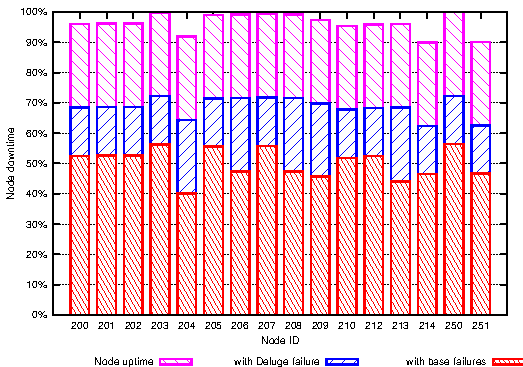
\includegraphics[width=\hsize]{./5-evaluation/figs/robustness/nodesalive/node-uptime2.pdf}
\end{center}
\caption{\textbf{Individual node uptimes.}
This figure shows the percentage of time that each node reported status
messages during the 19-day deployment.  Shown separately are the apparent
node uptimes caused by the whole-network outage and base station outages.
While the former was true sensor node failure, the latter did not seem to
affect the sensor nodes themselves.}
\end{figure}

Figure~\ref{evaluation-fig-nodeuptime} shows the uptime for each node during
the 19-day deployment. Each bar consists of three portions. The lowest
portion is the {\em apparent} uptime of each node accounting for both the
base station failures and single 3-day~software outage. Because base station
failures did not affect individual nodes, the middle bar shows the apparent
uptime including only the 3-day~outage. In this case, the mean node uptime
is~69\%.  However, with the 3-day outage factored out, nodes achieved an
average uptime of~96\%.  These numbers are encouraging and suggest that the
sensor nodes were very reliable in spite of the software crash.

Based on discussions with the authors of Deluge, we believe this failure was
caused by a single bug in the {\tt InternalFlash} TinyOS component (which has
since been fixed).  This bug prevented Deluge from storing critical state
information, causing nodes to reboot continuously at short intervals.  We did
not see this behavior in the lab before deployment, although we had not
rigorously tested this portion of the code. In retrospect, it was optimistic
of us to rely on a complex network reboot protocol that had not been
field-tested.  Deluge was removed from the binary used during the network
reprogram following the failure; it was replaced with a simpler mechanism to
reboot individual nodes using a radio command.

%  - Node reboots [KL]
%    - Determine manual vs. automatic reboots
%    - Correlate reboots to other node properties (routing load?)
%    - Impact of reboot (latency)
%\begin{figure}[t]
%  \begin{center}
%    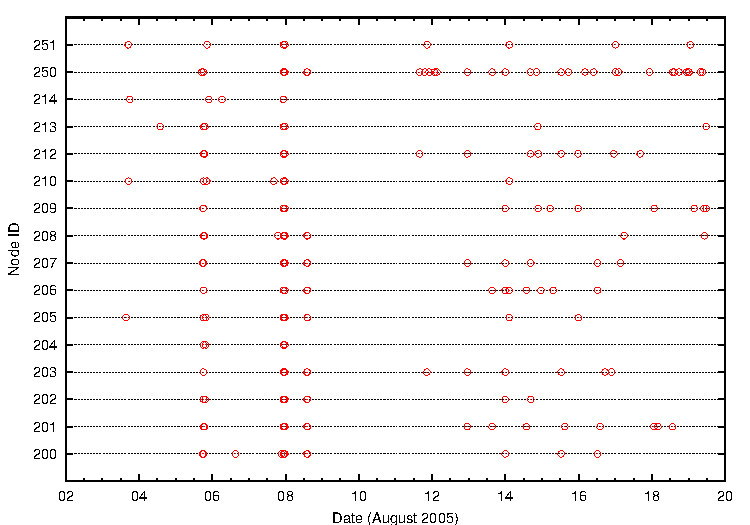
\includegraphics[width=\hsize]{./5-evaluation/figs/robustness/nodeReboots/nodeReboots.pdf}
%  \end{center}
%  \caption{\small{\bf Reboots of each node}
%    {\em This figure shows when each node rebooted during the 19-day deployment.}}
%    \label{fig-nodeReboots}
%\end{figure}


%\begin{figure}[t]
%  \begin{center}
%    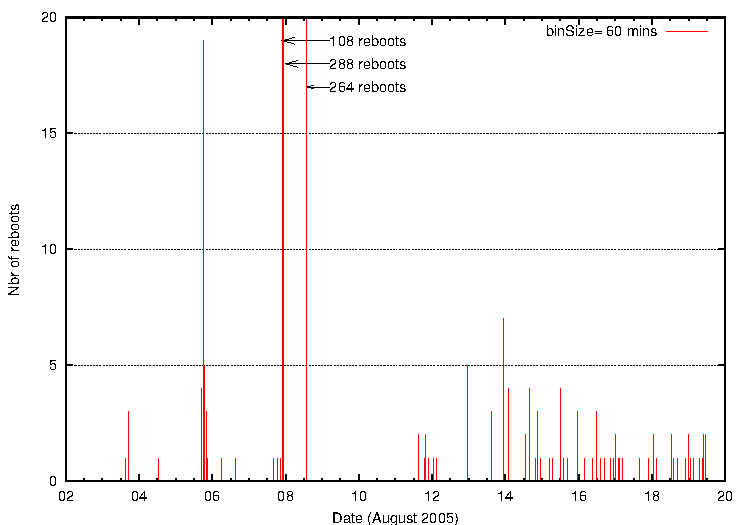
\includegraphics[width=\hsize]{./5-evaluation/figs/robustness/nodeReboots/nodeRebootsBinned.pdf}
%  \end{center}
%  \caption{\small{\bf Number of reboots over time}
%    {\em This figure shows a the number of reboots in 60 minute
%    windows.  As we can see, there was an unusually large number of
%    reboots right before the network reprogramming.}}
%    \label{fig-nodeRebootsBinned}
%\end{figure}

\subsection{Discussion}

Failures of the base station infrastructure were a significant source of
network downtime during the deployment.  This contrasts with common
assumptions that the base station is generally reliable and operating on a
continuous power source. This was our expectation prior to the deployment,
and we did not make adequate preparations for the intermittent electrical
supply at the observatory. A backup diesel generator was used during nightly
power outages, with extra laptop and car batteries supplying power when it
failed.  However, this approach was not ultimately successful.

It may be surprising that node uptime is not related to depth in the routing
tree. This suggests that if a node is ``down'' (i.e., we do not receive any
status messages from it during a 10-minute window) that it is still active
and routing packets for its children in the tree, even as its own status
messages are being lost. An alternate explanation is that a node could select
an alternate parent in the routing topology when its parent fails. However,
our analysis of the routing topology does not support this view, since nodes
rarely use more than one parent. For example, node~214 \textit{always} routes
data through node~251. The volcano-induced failure of node~204 near the end
of the deployment is the only notable failure of a single node.

